\chapter{Simulation par méthode spectrale}

\label{spectralMeth}
La méthode qui va être présentée est fondée essentiellement sur un cours de l'école Polytechnique (voir~\cite{FogliCoursX}). Le lecteur
est invité à lire l'annexe~\ref{annexeA} afin de mieux saisir les objets mathématiques utilisés dans ce chapitre.\\


Soit $(\Omega, F, \mathbb{P})$ un espace probabilisé, $n$ et $d$ deux entiers naturels non nuls et
$X = (X_1, \dots, X_d) : \mathbb{R}^n \times \Omega \rightarrow \mathbb{R}^d$ un champ aléatoire gaussien centré,
continue en moyenne quadratique et faiblement stationnaire d'ordre 2, admettant pour mesure spectrale $M_X$.
On supposera que $M_X$ admet une densité spectrale $S_X: \mathbb{R}^n \rightarrow M_d(\mathbb{R})$.\\

On va chercher à simuler $X$ sur un domaine appelé le domaine de simulation $\overline{T} = \overline{T_1} \times \dots \times \overline{T_n} $
un pavé de $\mathbb{R}^n$ où $\overline{T_j} = [0,T_j], \; T_j \in \mathbb{R}^{*}_{+}$. Une fois ce domaine défini, on discrétisera $\overline{T}$ en
une famille finie de points et on simulera $X$ en ces points que l'on appellera les points de simulation. \uppercase{à} la fin, on obtiendra un champ aléatoire gaussien
discret qui approchera $X$ sur $\overline{T}$.


\section{Hypothèses sur la densité spectrale}

Commençons en imposant trois hypothèses sur la densité spectrale $S_X$. Les deux premières hypothèses permettront de justifier mathématiquement le choix de la discrétisation du domaine de
simulation et la dernière permettra de construire l'algorithme de simulation de la méthode spectrale.
\begin{hypothesis}
$S_X$ est à support compact dans le pavé $\overline{\Omega} = \overline{\Omega_{1}} \times \dots \times \overline{\Omega_{n}}$ où $\forall j \in \llbracket 1; n \rrbracket , \; \overline{\Omega_{j}} = [-\Omega_{cj},\Omega_{cj}], \; \Omega_{cj} \in \mathbb{R}^{*}_{+}$ \label{hyp1}
\end{hypothesis}

\begin{hypothesis}
  $tr(S_X)$ est bornée (où $tr: M_d(\mathbb{\mathbb{C}}) \rightarrow \mathbb{C}$ est la fonction trace) \label{hyp2} 
\end{hypothesis}

\begin{hypothesis}
$\forall \omega \in \overline{\Omega} \setminus \partial\overline{\Omega}, \; S(\omega)$ est de rang $d$ (donc $S(\omega)$ est hermitienne définie positive)
\end{hypothesis}


\noindent En général, $S_X$ n'est pas forcément à support compact. Néanmoins:
\begin{itemize}
\item $\forall t \in \mathbb{R}^n, \mathbb{E}(\|X(t)\|_{2}^{2}) = \int_{\mathbb{R}^n} tr(S_X(\omega)) d\omega < \infty$ 
\item en pratique, $S_X(\omega)$ tend rapidement vers $ 0_{M_d(\mathbb{R})}$ quand $\|\omega \| \rightarrow \infty$ \\
\end{itemize}

\noindent Dans ces conditions on peut espérer trouver, pour $\epsilon \in \mathbb{R}^{*}_{+}$, arbitrairement petit, un pavé pas trop large $\overline{\Omega^{\epsilon}} = \overline{\Omega_{1}^{\epsilon}} \times \dots \times \overline{\Omega_{n}^{\epsilon}}$ tel que:
\begin{itemize}
\item $\forall j \in \llbracket 1; n \rrbracket$, $\overline{\Omega_{j}^{\epsilon}} = [-\Omega_{cj}^{\epsilon},\Omega_{cj}^{\epsilon}], \; \Omega_{cj}^{\epsilon} \in \mathbb{R}^{*}_{+}$
\item $ \int_{\mathbb{R}^n \setminus \overline{\Omega^{\epsilon}}} tr(S_X(\omega)) d\omega \leq (\int_{\mathbb{R}^n} tr(S_X(\omega)) d\omega) \cdot \epsilon$\\
\end{itemize}

Dans une telle configuration, on serait alors tenté d'approcher $S_X$ par $\mathds{1}_{\overline{\Omega^{\epsilon}}}S_X$ pour $\epsilon$ assez petit. D'où l'idée de chercher non pas à simuler le champ aléatoire $X$ directement mais à l'approcher par le champ aléatoire $X^{\epsilon}$ d'ordre 2, à valeurs dans $\mathbb{R}^d$, centré, gaussien, continue en moyenne quadratique, faiblement stationnaire d'ordre 2 et de
densité spectrale $\mathds{1}_{\overline{\Omega^{\epsilon}}}S_X$ (l'existence d'un champ gaussien à valeurs dans $\mathbb{R}^d$ de densité spectrale $\mathds{1}_{\overline{\Omega^{\epsilon}}}S_X$ peut se justifier mais on n'insistera pas sur ce point).
On revient ainsi au cas de $S_X$ à support compact. 

%à modifier

\section{Factorisation de Cholesky} 
\label{choleskyFactSection}
Pour $\omega$ dans $\overline{\Omega} \setminus \partial\overline{\Omega}$, $S_X(\omega)$ est hermitienne définie positive, donc admet une décomposition de Cholesky 
$S_X(\omega)=\mathcal{H}(\omega)\mathcal{H}(\omega)^{*}$ où $\mathcal{H}(\omega)$ est une matrice triangulaire inférieure. 
Une décomposition (non unique) de Cholesky peut s'obtenir à l'aide la méthode de Cholesky généralisée aux matrices hermitiennes définies-positives.

\section{Subdivision du domaine spectral}
\label{subdivdomspec}
Soit $N_1, \dots, N_n$, $n$ entiers naturels non nuls.
Imposons d'abord un certain nombre de notations:

\begin{itemize}
\item $N = N_1 \times \dots \times N_n$

\item pour $j \in \llbracket 1; N \rrbracket, \; B_{N_j} = \llbracket 1; N_j \rrbracket$

\item $B_N = B_{N_1} \times \dots \times B_{N_n}$ (produit cartésien)\\
\end{itemize}

Une arête $[-\Omega_{cj},\Omega_{cj}]$ sera subdivisée en $N_j$ intervalles réguliers $M_{j,1},\dots , M_{j,N_j}$ de longueur
\begin{equation}
 \Delta\omega_{j} = \frac{2\Omega_{cj}}{N_j}
\end{equation}
et de centres respectifs $\omega_{j,1}, \dots, \omega_{j,N_j}$.\\
\newpage
\noindent D'où plus explicitement pour $j \in \llbracket 1; n \rrbracket,\; k_j \in B_{N_j}$:
\begin{itemize}
\item $\omega_{j,k_j} = -\Omega_{cj} + (k_j - \frac{1}{2})\Delta\omega_{j} = (2k_j - 1 - N_j)\frac{\Delta\omega_{j}}{2}$ 

\item $M_{j,k_j} = [\omega_{j,k_j} - \frac{\Delta\omega_{j}}{2}, \omega_{j,k_j} + \frac{\Delta\omega_{j}}{2}]$\\
\end{itemize}

On peut ainsi définir une subdivision régulière de $\overline{\Omega}$ en $N$ mailles \mbox{\og carrés \fg} $M_k$ de centre $\omega_k$ de la façon suivante. 
Pour $k = (k_1, \dots, k_n) \in B_N$:
\begin{equation}
M_k = M_{1,k_1} \times \dots \times M_{n,k_n} 
%\end{equation} 
%\begin{equation} 
\quad \text{et} \quad \omega_k = (\omega_{1,k_1}, \dots, \omega_{n,k_n}) \label{mailles}
\end{equation}


\begin{figure}[h]
\begin{center}
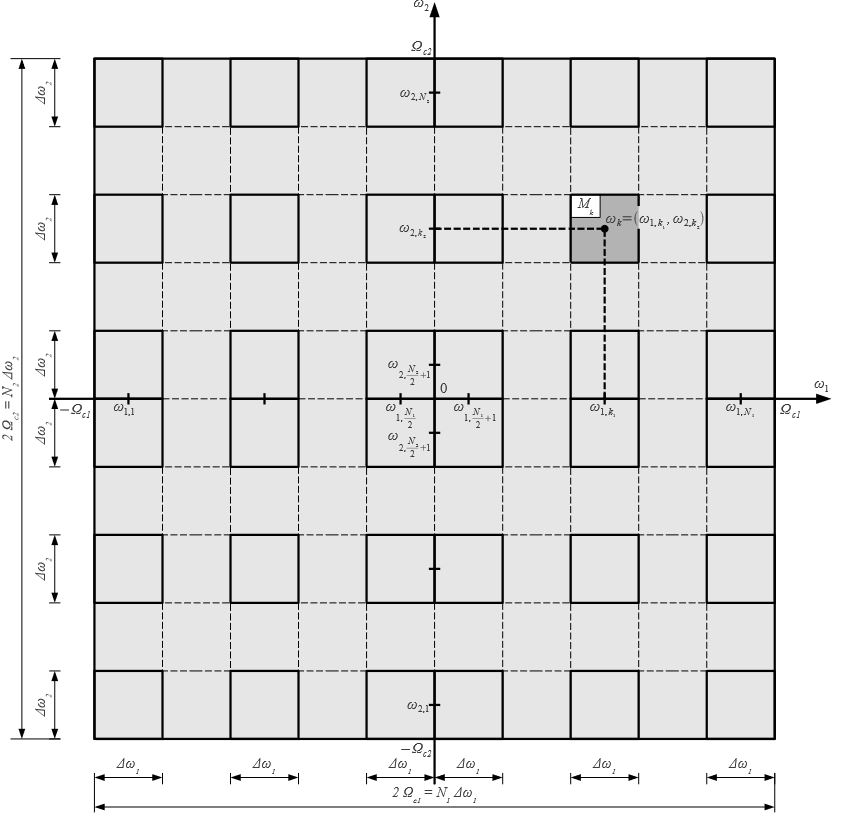
\includegraphics[scale=0.9]{images/grilleSpectraleDim2.jpg}
\caption{Subdivision du domaine spectral en dimension $n=2$}
\label{subdivSpecDim2}  
\end{center}
\end{figure}

\newpage
\begin{hypothesis}
  \label{symetrie} 
  Pour la suite, on supposera que les $N_j$ sont des multiples de 2. De cette façon, la subdivision $(M_k)_{k \in B_N}$ de $\overline{\Omega}$  est symétrique par rapport à l'origine (i.e si $\mathcal{S}$ est la symétrie de $\mathbb{R}^n$ qui à $x$ associe $-x$, alors $\mathcal{S}(\overline{\Omega}) = \overline{\Omega}$ et pour tout $k \in B_N$, il existe un unique $j \in B_N$ tel que $j \neq k$ et $\mathcal{S}(M_k) = M_j$ (on a même que $\omega_j = -\omega_k$)) et la famille des centres $(\omega_k)_{k \in B_N}$ ne contient pas l'origine $(0, \dots, 0)$. 
\end{hypothesis}




\section{Subdivision du domaine de simulation}
\label{subdiv}
On pose pour $j \in \llbracket 1; n \rrbracket, \; f_{max,j} = \frac{\Omega_{cj}}{2\pi}$. Il s'agit de la fréquence maximale sur l'arête spectrale $[-\Omega_{cj},\Omega_{cj}]$.\\

On obtient par le théorème d'échantillonage de Shannon, que pour $j \in \llbracket 1; n \rrbracket$ la fréquence d'échantillonage $f_{e,j}$ minimale requise pour représenter la densité spectrale $S_X$ sur le $j$\up{ème} axe de coordonnées vaut $2f_{max,j}$. Le pas d'échantillonage $\Delta t_{j}$ se définit alors ainsi:

\begin{equation} \forall j \in \llbracket 1; n \rrbracket , \; \Delta t_{j} = \frac{1}{f_{e,j}} = \frac{\pi}{\Omega_{cj}} \end{equation} 

\noindent On déduit alors la relation : pour $j \in \llbracket 1; n \rrbracket,\; \Delta t_{j}\Delta \omega_{j} = \frac{2\pi}{N_j}$.\\
Donc une fois que la discrétisation $(N_1, \dots, N_n)$ est donnée, le pas de pulsation $\Delta\omega_{j}$ et le pas de temps $\Delta t_{j}$ ne peuvent être choisis indépendamment.\\

Par ailleurs sous les hypothèses \ref{hyp1} et \ref{hyp2}, un théorème de Shannon plus fort garantit que la connaissance de $(X(k_1\Delta t_{1}, \dots, k_n\Delta t_{n}))_{(k_1, \dots, k_n) \in \mathbb{Z}^n}$ suffit pour déduire la loi du champ $X$ (voir page 446 de \cite{alma991000210539806616}). 

\noindent Par conséquent pour simuler un champ aléatoire approchant $X$, on pourra plutôt chercher à simuler un nombre fini de variables aléatoires de la famille $(X(k_1\Delta t_{1}, \dots, k_n\Delta t_{n}))_{(k_1, \dots, k_n) \in \mathbb{Z}^n}$. Explicitons lesquelles seront sélectionnées.\\

\noindent Posons pour $j \in \llbracket 1; n \rrbracket ,\; m_j \in \llbracket 1; N_j\rrbracket$:
\begin{itemize}
\item $t_{j,m_j} = (m_j - 1)\Delta t_{j}$
\item $T_j = N_j \Delta t_{j}$
\item $\overline{T_j} = [0, T_j]$


\item $\overline{T} = \overline{T_1} \times \dots \times \overline{T_n}$ (domaine de simulation)

\item pour $m \in B_N, t_m = (t_{1,m_1}, \dots, t_{n,m_n}) \in \overline{T}$ (points de simulation)\\
\end{itemize}

\begin{figure}[h]
\begin{center}
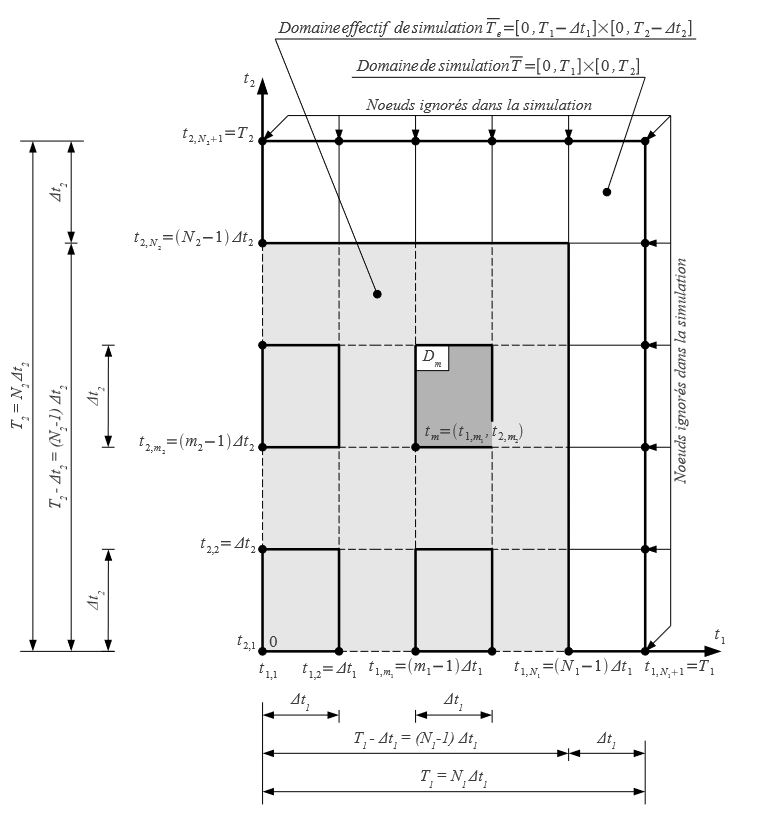
\includegraphics[scale=1.0]{images/MethSpect-domaineTemporelDeSimulationDim2.jpg}
\caption{Subdivision du domaine de simulation en dimension $n=2$}
\label{subdivSDomaineTempsDim2}  
\end{center}
\end{figure}

Avec ces notations, on peut maintenant dire que le but est de simuler la famille de vecteurs aléatoires $(X(t_m))_{m \in B_N}$ dont les éléments sont bien dans la
famille $(X(k_1\Delta t_{1}, \dots, k_n\Delta t_{n}))_{(k_1, \dots, k_n) \in \mathbb{Z}^n}$.


\section{Approximation du champ gaussien X}
\label{approxchmX}
$X$ est un champ d'ordre 2, centré, continue en moyenne quadratique et faiblement stationnaire d'ordre 2. On peut alors utiliser le théorème \ref{repSpec} de l'annexe \ref{annexeA}: on dispose de $\phi_X$, la mesure stochastique associée
à $X$ et issue de la mesure stochastique orthogonale centrée (m.s.o.c.) $I_X$
de mesure de base la mesure spectrale de $X$, $M_X$, telle que $\forall t \in \mathbb{R}^{n}$ :

\begin{equation}
X(t,.) = \displaystyle\int_{\mathbb{R}^n} \exp(i<t,\omega>_{n}) \phi_X(d\omega)= \displaystyle\int_{\overline{\Omega}} \exp(i<t,\omega>_{n}) \phi_X(d\omega) \label{specRepr}
\end{equation}

\begin{remark}
  La dernière égalité de la relation (\ref{specRepr}) se justifie par le support compact de $S_X$ dans $\overline{\Omega}$. En effet comme $M_X = S_X(\omega)d\omega$, on obtient que pour toute fonction $f$ dans $L^2(\mathbb{R}^n, M_X)$, $\|M_X\|$-presque partout, $f = \mathds{1}_{\overline{\Omega}} f$ (voir la définition~\ref{A22}). \\
\end{remark}

Or $\overline{\Omega}$ a été subdivisé par les mailles $M_k$ (voir la relation (\ref{mailles}))  et ces mailles sont à deux à deux disjointes (à un ensemble Lebesgue-négligeable près). D'où,
par linéarité de l'intégrale de Wiener et comme $X$ est à valeurs dans $\mathbb{R}^d$, pour $t \in \mathbb{R}^{n}$:
\begin{eqnarray}
X(t,.) &=& \displaystyle\sum_{k \in B_N} \displaystyle\int_{M_k} \exp(i<t,\omega>_{n}) \phi_X(d\omega) \notag{}\\
  &=& \mathfrak{Re}\biggl(\displaystyle\sum_{k \in B_N} \displaystyle\int_{M_k} exp(i<t,\omega>_{n}) \phi_X(d\omega)\biggr)
\end{eqnarray}

\`A partir de ce résultat, construisons peu à peu une approximation du processus $X$. On va d'abord faire l'approximation suivante:
~\\
\\$\forall t \in \mathbb{R}^{n}, \; \forall k \in B_N$,
\begin{eqnarray}
 \displaystyle\int_{M_k} \exp(i<t,\omega>_{n}) \phi_X(d\omega) &\approx& \displaystyle\int_{M_k} \exp(i<t,\omega_k>_{n}) \phi_X(d\omega) \notag{}\\
  &=& \exp(i<t,\omega_k>_{n}) \phi_X(M_k) 
\end{eqnarray}
\begin{remark}On peut y voir une quadrature par méthode du point milieu généralisée.\\\end{remark}

\noindent On obtient alors la première approximation de $X$ en posant pour $ t \in \mathbb{R}^{n}$: 

\begin{eqnarray}
Y(t,.) &=& \mathfrak{Re}\biggl(\displaystyle\sum_{k \in B_N} \exp(i<t,\omega_k>_{n}) \phi_X(M_k)\biggr) \notag{} \\
  &=& \mathfrak{Re}\biggl(I_X\biggl(\displaystyle\sum_{k \in B_N} \exp(i<t,\omega_k>_{n})\mathds{1}_{M_k}\biggl)\biggr) \notag{}
\end{eqnarray}

\noindent Pointons les propriétés suivantes (se justifiant à l'aide de la section~\ref{repSpecSect} de l'annexe \ref{annexeA}):
\begin{enumerate}
\item Comme $X$ est gaussien, les $\phi_X(M_k)$ sont des vecteurs gaussiens centrés de matrice de covariance complexe $\mathbb{E}(\phi_X(M_k)\phi_X(M_k)^{*}) = M_X(M_k) = \int_{M_k} S_X(\omega)d\omega$ 

\item Pour $(k,j) \in (B_N)^2,$ tel que $k \neq j,$ \\$  \; \mathbb{E}(\phi_X(M_k)\phi_X(M_j)^{*}) =  M_X(M_k \cap M_j) = 0_{M_d(\mathbb{C})}$.

\item Pour $(k,j) \in (B_N)^2, \; \mathbb{E}(\phi_X(M_k)\phi_X(M_j)^{\top}) = M_X(M_k \cap -(M_j))$

\item $Y$ est un champ gaussien centré \\
\end{enumerate}

\noindent Or par la symétrie de la subdivision $(M_k)_{k \in B_N}$ de $\overline{\Omega}$ (voir l'hypothèse~\ref{symetrie}), on a que pour tout $k \in B_N$, il existe un unique $j_k \in B_N$ différent de $k$ tel que $M_{j_k} = -M_k$. D'où:
\begin{equation}
  \label{five}
  \forall (k,l) \in (B_N)^2, \; \mathbb{E}(\phi_X(M_k)\phi_X(M_l)^{\top}) =
\begin{cases}
    M_X(M_k)    & \quad \text{si } l = j_k\\
    0_{M_d(\mathbb{C})}  & \quad \text{sinon }  \end{cases}
\end{equation}


\noindent $Y$ est un champ gaussien centré donc $Y$ est caractérisé par sa fonction de covariance que l'on note $C_Y: \mathbb{R}^n \times \mathbb{R}^n \rightarrow M_d(\mathbb{R})$. Par le calcul on obtient pour $(s,t) \in (\mathbb{R}^n)^2 :$
\begin{equation}
C_Y(s,t) = \mathbb{E}(Y(s)Y(t)^{\top}) = \mathfrak{Re}\biggl(\displaystyle\sum_{k \in B_N} e^{i<t-s,\omega_k>_n}M_X(M_k)\biggr)
\end{equation}

\noindent Ce résultat se fonde sur les propriétés 1, 2, 3, la formule~(\ref{five}) et sur la propriété suivante:
\begin{equation*}
\forall (A,B) \in M_{d,1}(\mathbb{C})^2, \; \mathfrak{Re}(A)\mathfrak{Re}(B)^{\top} = \frac{1}{2}(\mathfrak{Re}(AB^{\top}) + \mathfrak{Re}(AB^{*}))
\end{equation*}

\noindent Le souci devient alors les $(M_X(M_k))$ qui ont le défaut d'être définis par une intégrale. Cependant, en posant $\Delta\omega = \Delta\omega_1 \dots \Delta\omega_n$, on peut approcher les $M_X(M_k)$ ainsi: $ M_X(M_k) \approx \Delta\omega S_X(\omega_k)$ (encore une quadrature par méthode du point milieu généralisée).\\

On veut alors approcher le champ gaussien centré $Y$ par un champ gaussien centré dont la fonction de covariance vaut:
\begin{equation}
  K(s,t) = \Delta\omega \mathfrak{Re}\biggl(\displaystyle\sum_{k \in B_N} e^{i<t-s,\omega_k>_n}S_X(\omega_k)\biggr)
\end{equation}

 
\noindent Or on peut montrer que le champ $X_N$ suivant est à valeurs dans $\mathbb{R}^d$, gaussien, centré et que sa fonction de covariance vaut bien $K$:
\begin{equation}
  \forall t \in \mathbb{R}^n,\; X_N(t,.) = \mathfrak{Re}\biggl(\displaystyle\sum_{k \in B_N} \sqrt{\Delta\omega} \; e^{i<t,\omega_k>_{n}}\mathcal{H}(\omega_k)V_k \biggl) \label{formuleAppro}
\end{equation}
\noindent où:
\begin{itemize}
\item $\mathcal{H}(\omega)$ pour $\omega \in \overline{\Omega} \setminus \partial\overline{\Omega}$ a été définie plus tôt comme une factorisation de Cholesky (voir la section~\ref{choleskyFactSection})

\item les $(V_k)_{k \in B_N}$ sont des vecteurs gaussiens à valeurs dans $\mathbb{C}^d$ iid selon la loi normale centrée réduite complexe de $\mathbb{C}^d$ \\
\end{itemize}

\begin{remark}
  $\mathcal{H}(\omega_k)V_k $ est un produit matrice-vecteur
\end{remark}

\begin{remark}
\noindent $V$ un vecteur aléatoire à valeurs dans $\mathbb{C}^d$ suit la loi normale centrée réduite complexe si les parties réelle et imaginaire $\mathfrak{Re}(V)$ et $\mathfrak{Im}(V)$ suivent la loi normale centrée réduite de $\mathbb{R}^d$ et si $\mathfrak{Re}(V)$ et $\mathfrak{Im}(V)$ sont des vecteurs indépendants.
\end{remark}

Finalement on décide d'approcher le champ aléatoire $X$ par $X_N$ en les points de simulation $(t_m)_{m \in B_N}$ définis plus tôt (voir la section~\ref{subdiv}).
On cherche donc à simuler $(X_N(t_m,.))_{m \in B_N}$. Cette simulation est possible à l'aide d'un algorithme de simulation qui se déduit directement de la formule (\ref{formuleAppro}) du champ aléatoire $X_N$.

\section{Algorithme de simulation}

\subsection{Premier algorithme}
\label{firstone}
Pour modéliser les $(V_k)$ de la section précédente, il suffit de considérer $(U_{k,b,p})_{k \in B_N,  b \in \llbracket 0;1 \rrbracket, p \in \llbracket 1; d \rrbracket}$ une famille de $2\times Nd$ variables iid selon la loi normale centrée réduite de $\mathbb{R}$ et de poser pour $k \in B_N, V_k$ vecteur aléatoire à valeurs dans $\mathbb{C}^d$ tel que:
\begin{equation*}
  \mathfrak{Re}(V_k) = (U_{k,0,1}, \dots, U_{k,0,d}) \quad \text{et} \quad \mathfrak{Im}(V_k) = (U_{k,1,1}, \dots, U_{k,1,d})
\end{equation*}

\noindent On obtient alors l'algorithme de simulation suivant: 
\begin{itemize}
\item Soit $(u_{k,b,p})_{k \in B_N,  b \in \llbracket 0,1 \rrbracket, p \in \llbracket 1;d\rrbracket}$  une réalisation de taille $2\times Nd$ de la loi centrée réduite. 

\item On pose pour $k \in B_N, v_k \in \mathbb{C}^d$ tel que pour $p \in \llbracket 1;d\rrbracket$, la $p$-ième coordonnée de $v_k$ vaut $u_{k,0,p} + iu_{k,1,p}$

\item Pour $m \in B_N$ on pose:

   \begin{equation}x_N(t_m) = \mathfrak{Re}\biggl(\displaystyle\sum_{k \in B_N} \sqrt{\Delta\omega} \; e^{i<t_m,\omega_k>_{n}}\mathcal{H}(\omega_k)v_k \biggr) \label{formule1} \end{equation}

\end{itemize}


\noindent Les $x_N(t_m)$ constituent une réalisation du champ discret $(X_N(t_m))_{m \in B_N}$.


\subsection{Reformulation avec la densité spectrale fréquentielle}

Il est possible que l'on n'ait pas accès à la densité spectrale de $X$, $S_X$, mais à sa densité spectrale fréquentielle $S^{fr}_X$ (voir la sous-section~\ref{DSFr} de l'annexe~\ref{annexeA}). Dans ce cas, il est possible de reformuler l'algorithme de simulation en imposant quelques notations:\\

\begin{itemize}
\item  pour $k \in B_N, f_k = \frac{1}{2\pi} \cdot \omega_k \in \mathbb{R}^n \quad$ (fréquence associée aux $\omega_k$)
  
\item $\overline{D_f} = \frac{1}{2\pi}\overline{\Omega} = [-\frac{\Omega_{c1}}{2\pi},\frac{\Omega_{c1}}{2\pi}] \times \cdots \times [-\frac{\Omega_{cn}}{2\pi},\frac{\Omega_{cn}}{2\pi}]\quad$ (domaine fréquentiel)

\item $\forall j \in \llbracket 1; n \rrbracket, \; \Delta f_j = \frac{1}{2\pi}\Delta \omega_j $

\item $\Delta f = \Delta f_1 \dots \Delta f_n \in \mathbb{R}^{*}_{+}$ 

\item pour $f \in \overline{D_f} \setminus \partial \overline{D_f}, \; \tilde{H}(f) = (2\pi)^{\frac{n}{2}}\mathcal{H}(2\pi f) \quad$ ($2\pi f \in \overline{\Omega} \setminus \partial\overline{\Omega}$)\\

\end{itemize}

\noindent Remarquons d'abord que $\tilde{H}$ décrit une décomposition de Cholesky de $S^{fr}_X$:
\begin{equation*}
 \forall f \in \overline{D_f} \setminus \partial \overline{D_f}, \; \tilde{H}(f)\tilde{H}(f)^{*} = (2\pi)^{n}\mathcal{H}(2\pi f)\mathcal{H}(2\pi f)^{*} = (2\pi)^{n}S_X(2\pi f) = S^{fr}_X(f)
\end{equation*}

\noindent Une décomposition de Cholesky de $S^{fr}_X$ permet alors de réécrire les $x_N(t_m)$ introduits dans l'algorithme de simulation (voir la formule~(\ref{formule1})) à l'aide des notations posées juste avant:

\begin{equation*} \forall m \in B_N, \; x_N(t_m) = \mathfrak{Re}\biggl(\displaystyle\sum_{k \in B_N} \sqrt{\Delta f} \; e^{i<t_m,2\pi f_k>_{n}}\tilde{H}(f_k)v_k \biggl) \end{equation*}


\noindent Ce résultat indique la similitude des algorithmes de simulation peu importe si on voit le problème en fréquence ou en pulsation.


\subsection{Autre reformulation de l'approximation}

Dans l'annexe~\ref{annexeA}, on a exhibé multiples propriétés de la densité spectrale dont notamment celle-ci: $\forall \omega \in \mathbb{R}^n, \; S_X(-\omega) = \overline{S_X(\omega)}$. A partir de cette remarque, il est possible de décrire
un champ gaussien équivalent à $X_N$ (dans le sens où il suit la même loi que $X_N$).\\

\noindent Notons $A$ l'ensemble des $\omega_k$

\noindent Notons $B$ l'ensemble des $\omega_k$ tels que leur première coordonnée soit positive.

\noindent Notons $-B$ l'ensemble $\{ -b,\; b \in B\}$

\noindent On a supposé que les $(N_j)_{j \in \llbracket 1;n\rrbracket}$ étaient des multiples de $2$ (voir l'hypothèse~\ref{symetrie}). On a alors que $B$ est l'ensemble des $\omega_k$ tels que leur première coordonnée soit strictement positive. De façon plus explicite on a:
\begin{equation}
B = \{ \omega_k, \text{ où } k = (k_1, \dots, k_n) \in B_N \text{ et } k_1 \geq \frac{N_1}{2} + 1 \}
\end{equation}

\noindent Si on note  $\tilde{B} = \{ k = (k_1, \dots, k_n) \in B_N $ tel que $ k_1 \geq \frac{N_1}{2} + 1 \} $, on montre aussi que:
\begin{eqnarray*}
  A \setminus B &=& \{ \omega_{(N_1-k_1+1, N_2-k_2+1, \dots, N_n-k_n+1)} \text{ où } k = (k_1, \dots, k_n) \in \tilde{B} \}\\
  &=& \{ -\omega_k \text{ où } k = (k_1, \dots, k_n) \in \tilde{B} \}\\
  &=& -B
\end{eqnarray*}

\newpage
D'où le couple $(B,-B)$ forme une partition de $A$ l'ensemble des $\omega_k$. Il
est alors possible de réécrire la formule (\ref{formuleAppro}) du champ $X_N$. Si on pose pour $k = (k_1, \dots, k_n) \in B_N, \; j_k = (N_1-k_1+1, N_2-k_2+1, \dots, N_n-k_n+1)$,
alors pour $t \in \mathbb{R}^n$:

\begin{eqnarray*}
X_N(t, .) &=&  \mathfrak{Re}\biggl(\displaystyle\sum_{k \in B_N} \sqrt{\Delta\omega} \; e^{i<t,\omega_k>_{n}}\mathcal{H}(\omega_k)V_k\biggr) \\
&=& \mathfrak{Re}\biggl(\displaystyle\sum_{k = (k_1,\dots, k_n) \in \tilde{B}} \sqrt{\Delta\omega} \;( e^{i<t,\omega_k>_{n}}\mathcal{H}(\omega_k)V_k + e^{i<t,\omega_{j_k}>_{n}}\mathcal{H}(\omega_{j_k})V_{j_k}) \biggl) \\
&=& \mathfrak{Re}\biggl(\displaystyle\sum_{k = (k_1,\dots, k_n) \in \tilde{B}} \sqrt{\Delta\omega} \;( e^{i<t,\omega_k>_{n}}\mathcal{H}(\omega_k)V_k + e^{i<t,-\omega_k>_{n}}\overline{\mathcal{H}(\omega_k)}V_{j_k})\biggl) \\
&=& \mathfrak{Re}\biggl(\displaystyle\sum_{k = (k_1,\dots, k_n) \in \tilde{B}} \sqrt{\Delta\omega} \;( e^{i<t,\omega_k>_{n}}\mathcal{H}(\omega_k)V_k + \overline{e^{i<t,\omega_k>_{n}}\mathcal{H}(\omega_k)\overline{V_{j_k}}}) \biggl) \\
\end{eqnarray*}



\begin{remark}
  La notation $j_k$ est la définition explicite de la notation $j_k$ introduite à la section~\ref{approxchmX} et utilisée pour la formule~(\ref{five}).
\end{remark}


On observe que $\overline{V_{j_k}}$ suit la même loi que $V_{j_k}$ et plus généralement que la famille de vecteurs aléatoires composée de ceux de la famille $(V_k)_{k \in \tilde{B}}$ et de ceux de la famille $(\overline{V_{j_k}})_{k \in \tilde{B}}$ forme une famille de variables aléatoires iid qui peut être confondue avec la famille $(V_k)_{k \in B_N}$. Donc si on pose pour $t \in \mathbb{R}^n$:

\footnotesize{
\begin{equation}
\tilde{X}_N(t, .) =  \mathfrak{Re}\biggl(\displaystyle\sum_{k = (k_1,\dots, k_n) \in \tilde{B}} \sqrt{\Delta\omega} \;( e^{i<t,\omega_k>_{n}}\mathcal{H}(\omega_k)V_k + \overline{e^{i<t,\omega_k>_{n}}\mathcal{H}(\omega_k)V_{j_k}}) \biggr)\\
\end{equation}
}

\normalsize{
  \noindent alors ce champ $\tilde{X}_N$ suit la même loi que le champ $X_N$. Par conséquent, en raisonnant comme à la sous-section~\ref{firstone}, on peut en déduire sans souci un deuxième algorithme
  pour simuler les $(\tilde{X}_N(t_m))_{m \in B_N}$. L'avantage de ce nouvel algorithme sera de diminuer les calculs. En effet la connaissance des $(\mathcal{H}(\omega_k))_{k \in \tilde{B}}$, qui s'obtiennent
  par la méthode de Cholesky, suffit. D'où 2 fois moins de calculs ($\tilde{B}$ est de cardinal $N/2$).}


\section{Algorithme de simulation et TFD}

Si on reconsidère dans la sous-section~\ref{firstone}, la formule~(\ref{formule1}) des $x_N(t_m)$ qui décrit le premier algorithme de simulation, la formule se veut sous une forme
matricielle très condensée. De plus cette formule n'utilise pas la définition des $t_m$ et des $\omega_k$ (voir les sections~\ref{subdivdomspec} et~\ref{subdiv})
. Il est donc intéressant de développer la formule des $x_N(t_m)$ pour chaque coordonnée $p$ allant de $1$ à $d$ (que l'on va noter $x_{N,p}(t_m)$)
Dans cette section, on met en avant la présence d'une transformée de
Fourier discrète (TFD), dont l'algorithme associé se veut particulièrement efficace.\\


\noindent Pour $m \in B_N$ et $k \in B_N$, on obtient en développant le produit scalaire suivant:
\begin{eqnarray*}
  <t_m,\omega_k>_{n} \; &=&  \; \displaystyle\sum_{j = 1}^{n} t_{j,m_j} \omega_{j,k_j} \\ 
  &=& \; \displaystyle\sum_{j = 1}^{n} \biggl( -\frac{\pi (m_j - 1)(N_j - 1)}{N_j} + \frac{2\pi(m_j - 1)(k_j -1)}{N_j} \biggr)
\end{eqnarray*}
 
~\\
\noindent Si on utilise cette formule dans la formule des $x_N(t_m)$, on obtient alors pour $m \in B_N$ et $p \in \llbracket 1;d \rrbracket$ :

\begin{equation*}
  x_{N,p}(t_m) = \sqrt{\Delta \omega} \; \mathfrak{Re} \biggl (y_{N,p}(m) \cdot \exp \biggl(-i \pi \displaystyle\sum_{j = 1}^{n} \frac{(m_j - 1)(N_j - 1)}{N_j} \biggr) \biggr)  
\end{equation*}

\noindent où:
\begin{itemize}

\item $y_{N,p}(m) = \displaystyle\sum_{k \in B_N}  z_{p}(k) \cdot \exp \biggl(2i\pi \displaystyle\sum_{j = 1}^{n} \frac{(m_j - 1)(k_j -1)}{N_j} \biggr)$\\
~\\
\item $z_{p}(k) \; = \; \displaystyle\sum_{q = 1}^{d} \mathcal{H}_{pq}(\omega_k) \cdot (u_{k,0,q} + i.u_{k,1,q}) \;$ pour $k \in B_N$\\
\end{itemize}
~\\
On observe pour $p \in \llbracket 1;d \rrbracket$ que la famille $(y_{N,p}(m))_{m \in B_N}$ n'est rien d'autre que
la transformée de Fourier discrète (TFD) de la famille $(z_{p}(k))_{k \in B_N}$.\\
De façon générale si $n \in \llbracket 1;3 \rrbracket$, l'algorithme de simulation admet une complexité en temps en $O(d Nlog(N)+d^3 N)$ à cause 
des $d$ TFDs et du calcul des factorisations de Cholesky. Comme $d$ varie en général entre $1$ et $3$
on peut parler d'une complexité en $O(Nlog(N))$). La complexité en mémoire est en  $O(d^2 N)$, en raison du
stockage des $N$ factorisations de Cholesky. 


\section{Propriétés des approximations $X_N$}

Dans cette section, on répertorie un ensemble de propriétés vérifiées
par l'approximation du champ gaussien $X$, $X_N$, introduit à la section~\ref{approxchmX} par la formule~\ref{formuleAppro}.\\

\begin{itemize}
  \item $X_N$ est un champ gaussien centré, homogène tel que:
   \begin{equation}
    \mathbb{E}(\|X_N\|_{2}^{2}) \; = \; \Delta \omega \cdot \displaystyle\sum_{k \in B_N} tr(S_X(\omega_k))    
   \end{equation}

 \item Si on note $R_{X_N}$ sa fonction d'autocovariance qui à $s \in \mathbb{R}^n$ associe $\mathbb{E}(X_N(0)X_N(s))^{T}$, alors:
   \begin{equation}
    R_{X_N}(s) = \Delta\omega \cdot \mathfrak{Re}\biggl (\displaystyle\sum_{k \in B_N} e^{i<s,\omega_k>_n}S_X(\omega_k)\biggr)  \label{autocov}  
   \end{equation}

   \noindent On remarque que $\displaystyle\sum_{k \in B_N} e^{i<s,\omega_k>_n}S_X(\omega_k)$ est un réel \\

 \item $X_N$ est continue en moyenne quadratique et admet une mesure spectrale $M_{X_N}$ à valeurs dans $M_d(\mathbb{R})$ tel que:
   \begin{equation}
     M_{X_N} = \Delta\omega \cdot \displaystyle\sum_{k \in B_N} S_X(\omega_k)\delta_{\omega_k} \label{mesSpec}
   \end{equation}
   où $\delta_{\omega_k}$ est la mesure de Dirac en $\omega_k$ (mesure sur $(\mathbb{R}^n,\mathcal{B}(\mathbb{R}^n)$)\\

 \item $X_N$ est presque sûrement à trajectoires continues.\\

 \item Les trajectoires de $X_N$ sont de période $\tau = (\tau_1, \cdots, \tau_n)$\\
   où $\forall j \in \llbracket 1;n \rrbracket, \; \tau_j = \frac{4\pi}{\Delta \omega_j} = 2T_j$
   (i.e $\forall j \in \llbracket 1;n \rrbracket, \; \forall t \in \mathbb{R}^n, \; \\ X_N(t_1, \cdots, t_j + \tau_j, \cdots, t_n) = X_N(t_1, \cdots, t_j, \cdots, t_n)$)
\end{itemize}
~\\

Considérons maintenant une suite $( N^{j} = (N_1^{j}, \cdots, N_n^{j}))_{j \in \mathbb{N}}$ à valeurs dans $\mathbb{N}^n$. Pour $j \in \mathbb{N}$, on note $N_{inf}^{j} = \displaystyle\inf_{i \in \llbracket 1;n \rrbracket} N_i^{j}$. On suppose que $N_{inf}^{j} \underset{j \to \infty}{\to} \infty$.\\

\noindent Notons maintenant pour $j \in \mathbb{N}$,  $X_{N^j}$ le champ aléatoire défini par la formule~(\ref{formuleAppro}), $M_{X_{N^{j}}}$ sa mesure spectrale définie par
la formule~\ref{mesSpec} et $R_{X_{N^{j}}}$ la fonction d'autocovariance de $X_{N^j}$ définie par la formule~(\ref{autocov})
où dans les formules la discrétisation $(N_1, \cdots, N_n)$ qui définit les $\omega_k$
est remplacée par la discrétisation $(N_1^{j}, \cdots, N_n^{j})$.\\

\noindent On obtient alors des propriétés de convergence:\\


\begin{itemize}
\item La suite $(X_{N^j})_{j \in \mathbb{N}}$ converge en loi vers le champ aléatoire $X$.
\item La suite $(R_{N^j})_{j \in \mathbb{N}}$ converge uniformément dans tout compact de $\mathbb{R}^n$ vers $R_X$ la fonction d'autocovariance de $X$.
\item Pour tout $(k,l) \in \llbracket 1;d \rrbracket^2$, la suite de mesures complexes $((M_{N^j})_{k,l})_{j \in \mathbb{N}}$ converge étroitement vers la mesure $(M_X)_{k,l}$ 
\item Si $S_X$ est de classe $C^1$ (resp. $C^2$) sur $\overline{\Omega}$, alors la vitesse des 2 convergences précédentes est en $(N_{inf}^{j})^{-1}$ (resp. $(N_{inf}^{j})^{-2}$).
\end{itemize}

\section{Erreur et convergence numérique}
\label{erreurConvSpectral}
\subsection{Nouvel estimateur}

Dans le cas de la méthode spectrale, on ne choisira pas d'estimer
l'erreur $L^2$ de $N$ réalisations (voir la sous-section~\ref{quantifErreur}
du chapitre \ref{chapCholesky}) afin de valider cette méthode
de simulation. On rappelle que l'erreur $L^2$ permet de voir à quel point
par $N$ réalisations, on approche la matrice de covariance $\Sigma$ du problème. Or
même si à partir d'une densité spectrale on peut obtenir par calcul la fonction
d'autocovariance d'un processus (et donc la fonction de covariance dont on déduit la matrice $\Sigma$), on
peut être dans une situation où seule l'information de la densité spectrale
est disponible. C'est donc cette dernière que l'on cherchera à estimer à
l'aide de $L$ réalisations indépendantes du même processus sur le domaine
de simulation. Explicitons l'estimateur évoqué dans la référence~\cite{FogliCoursX}.\\

Soit $(x^{(1)}(t_m))_{m \in B_N}, \cdots, (x^{(L)}(t_m))_{m \in B_N} $ $L$ réalisations indépendantes du
processus $X_N$ (voir la formule (\ref{formuleAppro}) de la section~\ref{approxchmX}) en les points de simulation $(t_m)_{m \in B_N}$ (voir
la section~\ref{subdiv}). Pour valider nos simulations, on décide d'utiliser plus précisement un estimateur de la densité spectrale fréquentielle $S_X^{fr}$ en les
points $(f_k)_{k \in B_N}=(\frac{1}{2\pi}\omega_k)_{k \in B_N}$ (voir formule~(\ref{mailles}) de la section~\ref{subdivdomspec}) que l'on qualifiera de points fréquentiels associés aux points de simulation.
On définit alors pour $k = (k_1, \cdots, k_n) \in B_N$ l'estimateur de $S_X^{fr}(f_k)$ :
\begin{equation}
\hat{S}(f_k) = \frac{1}{L} \displaystyle\sum_{l = 1}^{L} \hat{Z}^{(l)}(k)\hat{Z}^{(l)}(k)^{*} \in M_d(\mathbb{C})  
\end{equation}

où:

\begin{itemize}

\item pour $l \in \llbracket 1;L \rrbracket$, $\hat{Z}^{(l)}(k) = (\hat{Z}^{(l)}_{1}(k), \cdots, \hat{Z}^{(l)}_{d}(k))^{T}$\\
  
\item pour $l \in \llbracket 1;L \rrbracket$, pour $p \in \llbracket 1;d \rrbracket$:
  \begin{equation*} \hat{Z}^{(l)}_{p}(k) = \displaystyle\sum_{m \in B_N} Z_{p}^{(l)}(m)\cdot\exp \biggl(-2i\pi \displaystyle\sum_{j = 1}^{n} \frac{(m_j -1)(k_j -1)}{N_j} \biggr)  \end{equation*}

\item pour $l \in \llbracket 1;L \rrbracket$, $m \in B_N $ et  $p \in \llbracket 1;d \rrbracket$:
  \begin{equation*} Z^{(l)}_{p}(m) = \Delta t \cdot W_{\bar{T}}(t_m) \cdot x^{(l)}_{p}(t_m) \cdot \exp \biggl (i\pi \displaystyle\sum_{j = 1}^{n} \frac{(m_j -1)(N_j -1)}{N_j} \biggr)  \end{equation*}

\item pour $s \in \mathbb{R}^{n}, W_{\bar{T}}(s) = W_{T_1}(s_1) \cdots W_{T_n}(s_n)$ (on parle de fenêtre temporelle de dimension $n$ sur $\bar{T} = [0,T_1] \times \cdots \times [0,T_n]$) \\

\item pour $s \in \mathbb{R}$ et $j \in \llbracket 1;n \rrbracket$, $W_{T_j}(s) = \frac{1}{\sqrt{T_j}} W(\frac{s}{T_j})$ où
$W$ est une fenêtre temporelle de dimension $1$ standard.
\end{itemize}

\begin{definition}
  Une fenêtre temporelle d'énergie normalisée standard ou juste fenêtre temporelle de dimension $1$ standard est une fonction $W: \mathbb{R} \rightarrow \mathbb{R}$ mesurable telle que:
\begin{itemize}
\item $supp(W) \subset [0,1]$ (support de $W$ inclus dans $[0,1]$)
\item $W(1-t) = W(t)$ pour $t \in \mathbb{R}$
\item $\displaystyle\int_{\mathbb{R}} W(t)^2 dt = \displaystyle\int_{0}^{1} W(t)^2 dt = 1$
\item si on note $\hat{W}$ la transformée de Fourier de $W$
et que l'on note pour $T \in \mathbb{R}^{*}_{+}$ et $\omega \in \mathbb{R}$, $G_{T}(\omega) = \frac{T}{2\pi} |\hat{W}(T\omega)|^{2}$, alors
quand $T$ tend vers l'infini, $G_T$ converge en distribution vers la masse de Dirac en $0$.
\end{itemize}
\end{definition}

\begin{remark}
  $\hat{W}(\omega) = \displaystyle\int_{\mathbb{R}} e^{-i\omega t} W(t) dt $
\end{remark}
%~\\
\begin{remark}
  Pour $T \in \mathbb{R}^{*}_{+}$, $W_{T}: t \rightarrow \frac{1}{\sqrt{T}} W(\frac{t}{T}) $ est appelé fenêtre temporelle et
  vérifie les propriétés suivantes:
  \begin{itemize}
   \item $supp(W_T) \subset [0,T]$ 
   \item $W_T(T-t) = W_{T}(t)$ pour $t \in \mathbb{R}$
   \item $\displaystyle\int_{\mathbb{R}} W_T(t)^2 dt = \displaystyle\int_{0}^{T} W_T(t)^2 dt = 1$
   \item $\frac{1}{2\pi} |\hat{W_T}(\omega)|^{2} = G_{T}(\omega)$ pour $\omega \in \mathbb{R}$
     (on dit alors que $G_{T}$ est la fenêtre spectrale associée à $W_{T}$)
\end{itemize}
\end{remark}

\noindent Dans la référence~\cite{alma991000210539806616}, plus de détails sur les fenêtres temporelles sont évoqués
et leur rôle est d'essayer d'améliorer les estimations d'une densité spectrale. On peut citer comme exemple de
fenêtre temporelle standard, la fenêtre de Hamming que l'on utilisera pour nos tests numériques et qui est
définie de la façon suivante pour $t \in \mathbb{R}$:

\begin{equation} W(t) = 1.5863 \;(0.54 - 0.46\cos(2\pi t))\;\mathds{1}_{[0,1]}(t) \end{equation}

Dans les références~\cite{FogliCoursX} et~\cite{alma991000210539806616} , la pertinence (dans le cas des champs gaussiens surtout)
d'utiliser un tel estimateur pour la densité spectrale $S_X^{fr}$ en augmentant le nombre de réalisations $L$
y est un peu plus développé mais on n'entrera pas dans les détails.\\

Finalement on quantifie l'erreur de simulation en définissant l'erreur absolue $\epsilon$ suivante:
\begin{equation}  \epsilon = \max_{k \in B_N} \|\hat{S}(f_k) - S_X^{fr}(f_k)\|_{F}  \label{errAbs}\end{equation}

\subsection{Résultats numériques}

Dans l'annexe~\ref{codeNumAnnexe}, dans la section~\ref{dossSpec}, plusieurs
densités spectrales y sont évoquées et ont une notation: \eqref{S1} et sa fonction d'autocovariance associée \eqref{R1}, \eqref{S2}
et sa fonction d'autocovariance associée \eqref{R2}, etc... On utilisera cette notation afin de les désigner par la suite.
Par ailleurs  on maintient toujours les notations utilisées jusqu'à maintenant pour décrire la
méthode spectrale: $N_1, \cdots, N_n, f_{max,1}, \cdots, f_{max,n}$ et ainsi de suite. Pour nos tests, $n \in \llbracket 1;3 \rrbracket$ et
bien qu'il ne soit pas nécessaire d'associer un maillage aux points de simulation, en raison de la répartition régulière dans l'espace
des points de simulation, on peut y associer tout de même un maillage
triangulaire dont les n\oe uds sont les points de simulations et dont les $n$-simplexes sont définis de la même façon que pour les maillages
évoqués à la section~\ref{errConvCholesky} du chapitre~\ref{chapCholesky}.\\


Les sous-sous-sections suivantes décrivent les différents tests numériques effectués. Ces derniers sont contenus dans le fichier spectral.py (voir la section~\ref{dossSpec} de
l'annexe~\ref{codeNumAnnexe}). Pour tester l'estimateur de densité spectrale, il a fallu choisir le nombre de réalisations indépendantes $L$
du processus $X_N$ et on l'a fait varier entre $100$ et $2000$. L'erreur de simulation sera l'erreur absolue $\epsilon$
décrite par la formule~\eqref{errAbs}. Pour le choix de la fenêtre temporelle
standard, on opte pour la fenêtre de Hamming.

\subsubsection{Dimension n=1}
En dimension 1, on a choisi la densité spectrale (fréquentielle)~\eqref{S1} où le paramètre $A$ a été
fixé à 5.0. Comme la densité~\eqref{S1} est à support dans $[-A,A]$, il est pertinent de choisir $f_{max,1} = A$.
Le nombre de points de simulation $N = N_1$ varie entre $10$ et $10000$. La connaissance de $N$ et $f_{max,1}$ permet
de déduire les $N$ points de simulation $(\frac{m-1}{2f_{max,1}})_{m \in \llbracket 1;N \rrbracket}$. Le point de simulation de valeur maximale est
donc le point $t_{N} = \frac{N-1}{2f_{max,1}}$, qui est le temps effectif de simulation en constraste avec le temps de simulation
$T_1 = \frac{N}{2f_{max,1}}$. Aux points de simulation, on associe les points fréquentiels:
\begin{equation*} \biggl((2i -1 - N) \frac{f_{max,1}}{N_1}\biggr)_{i \in \llbracket 1;N \rrbracket} \end{equation*}

\subsubsection{Dimension n=2}
En dimension 2, on a choisi la densité spectrale~\eqref{S4} où le paramètre $\sigma$ vaut $1$ et les paramètres $b_1$ et $b_2$ ont été
fixés respectivement à $1$ et $4$. On a fixé $f_{max,1} = \frac{20}{2\pi}$ et  $f_{max,2} = \frac{5}{2\pi}$.
Le nombre de points de simulation $N = N_1 \times N_2$ varie entre $10$ et $10000$ et $N_1 = N_2$. La connaissance de $N$, $f_{max,1}$ et $f_{max,2}$  permet
de déduire les $N$ points de simulation: \begin{equation*} \biggl(\biggl(\frac{i-1}{2f_{max,1}},\frac{j-1}{2f_{max,2}}\biggr)\biggr)_{(i,j) \in \llbracket 1;N_1 \rrbracket \times \llbracket 1;N_2 \rrbracket } \end{equation*}
auxquels on associe les points fréquentiels:
\begin{equation*} \biggl(\biggl((2i -1 - N_1) \frac{f_{max,1}}{N_1}, (2j -1 - N_1) \frac{f_{max,2}}{N_2}\biggr)\biggr)_{(i,j) \in \llbracket 1;N_1 \rrbracket \times \llbracket 1;N_2 \rrbracket } \end{equation*}

\subsubsection{Dimension n=3}
En dimension 3, on a choisi la densité spectrale~\eqref{S3} où le paramètre $a$ a été fixé à $1.0$. Les fréquences maximales
$f_{max,1}, f_{max,2}, f_{max,3}$ ont été fixées toutes trois à $10$.
Le nombre de points de simulation $N = N_1 \times N_2 \times N_3$ varie entre $10$ et $10000$ et  $N_1 = N_2 = N_3 $. La connaissance de $N$, $f_{max,1}$, $f_{max,2}$ et $f_{max,3}$ permet
de déduire les $N$ points de simulation:
\begin{equation*} \biggl (\biggl(\frac{i-1}{2f_{max,1}},\frac{j-1}{2f_{max,2}},\frac{k-1}{2f_{max,3}}\biggr)\biggr)_{(i,j,k) \in \llbracket 1;N_1 \rrbracket \times \llbracket 1;N_2 \rrbracket \times \llbracket 1;N_3 \rrbracket} \end{equation*} 
auquels on associe les points fréquentiels:
\small{
\begin{equation*}  \biggl(\biggl((2i -1 - N_1) \frac{f_{max,1}}{N_1}, (2j -1 - N_1) \frac{f_{max,2}}{N_2},(2k -1 - N_1) \frac{f_{max,3}}{N_3}\biggr)\biggr)_{(i,j,k) \in \llbracket 1;N_1 \rrbracket \times \llbracket 1;N_2 \rrbracket \times \llbracket 1;N_3 \rrbracket} \end{equation*}
}

\normalsize{}

\subsubsection{Benchmarks}

\phantom{
\noindent espace\\
espace\\
}

\begin{table}[htbp]
  \centering
\begin{tabular}{|>{\centering\arraybackslash}p{1.7cm} |>{\centering\arraybackslash}p{1cm} |>{\centering\arraybackslash}p{7cm} |}
\hline
Dimension & Nb de n\oe uds $N$ & Temps moyen d'une réalisation (en seconde) \\
\hline
1 & 10 & 0.00024s    \\
\hline
1 & 100 & 0.00196s  \\
\hline
1 & 1000 & 0.01924s   \\
\hline
1 & 10000 & 0.19921s    \\
\hline
\hline
2 & 16 & 0.00060s    \\
\hline
2 & 100 & 0.00271s    \\
\hline
2 & 1024 & 0.02546s  \\
\hline
2 & 10000 & 0.24736s   \\
\hline
\hline
3 & 8 & 0.00040s    \\
\hline
3 & 64 & 0.00200s    \\
\hline
3 & 1000 & 0.02714s    \\
\hline
3 & 10648 & 0.27015s  \\
\hline
\end{tabular}
\end{table}

\begin{table}[htbp]
  \centering
\begin{tabular}{|c |c |c |c |c |}
\hline
Dimension & Nb de n\oe uds $N$  & Nb de réalisations $L$ & erreur $\epsilon$ \\
\hline
1 & 100 & 100 & 0.02323   \\
\hline
1 & 100 & 500 & 0.00803    \\
\hline
1 & 100 & 1000 & 0.00968    \\
\hline
1 & 100 & 2000 & 0.00485    \\
\hline
\hline
1 & 500 & 100 & 0.02758    \\
\hline
1 & 500 & 500 & 0.01412  \\
\hline
1 & 500 & 1000 & 0.00815    \\
\hline
1 & 500 & 2000 & 0.00835    \\
\hline
\hline
1 & 1000 & 100 & 0.03043    \\
\hline
1 & 1000 & 500 & 0.01536    \\
\hline
1 & 1000 & 1000 & 0.01083   \\
\hline
1 & 1000 & 2000 & 0.00751    \\
\hline
\hline
\hline
2 & 100 & 100 & 0.56987   \\
\hline
2 & 100 & 500 & 0.39173    \\
\hline
2 & 100 & 1000 & 0.42713    \\
\hline
2 & 100 & 2000 & 0.45083    \\
\hline
\hline
2 & 484 & 100 & 5.07162    \\
\hline
2 & 484 & 500 & 2.54857   \\
\hline
2 & 484 & 1000 & 2.94699    \\
\hline
2 & 484 & 2000 & 3.13654  \\
\hline
\hline
2 & 1024 & 100 & 2.01205    \\
\hline
2 & 1024 & 500 & 1.83634    \\
\hline
2 & 1024 & 1000 & 0.93156    \\
\hline
2 & 1024 & 2000 & 1.05494    \\
\hline
\hline
\hline
3 & 64 & 100 & 1.80454.$10^{-5}$   \\
\hline
3 & 64 & 500 & 1.66974.$10^{-5}$    \\
\hline
3 & 64 & 1000 & 1.62478.$10^{-5}$    \\
\hline
3 & 64 & 2000 & 1.52534.$10^{-5}$    \\
\hline
\hline
3 & 512 & 100 & 0.00027    \\
\hline
3 & 512 & 500 & 0.00024   \\
\hline
3 & 512 & 1000 & 0.00021    \\
\hline
3 & 512 & 2000 & 0.00022    \\
\hline
\hline
3 & 1000 & 100 & 0.00065    \\
\hline
3 & 1000 & 500 & 0.00062    \\
\hline
3 & 1000 & 1000 & 0.00054    \\
\hline
3 & 1000 & 2000 & 0.00057    \\
\hline
\end{tabular}
\end{table}
\newpage


\begin{remark}
  Dans le tableau de l'erreur $\epsilon$, l'erreur ne décroît pas forcément bien vers $0$ et certains niveaux d'erreur
  sont étonnamment élevés (dimension 2). On soupçonne un bug qui est toujours en cours d'investigation au moment de la
  rédaction du rapport.
\end{remark}

\phantom{oyez}\\
\phantom{oyez}\\

\begin{figure}[h]
\centering
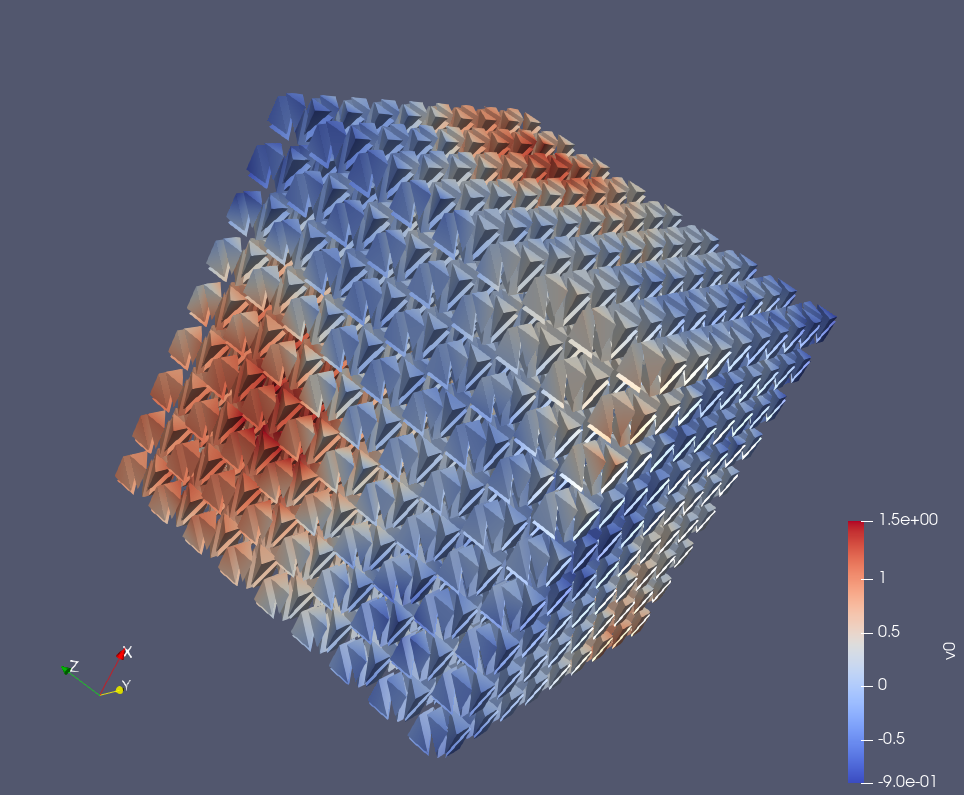
\includegraphics[scale=0.4]{images/meshSpectral3D-1000.png}
\caption{Réalisation en dimension 3 où $N = 1000$ }
\label{ReaDim2-961}  

\end{figure}
